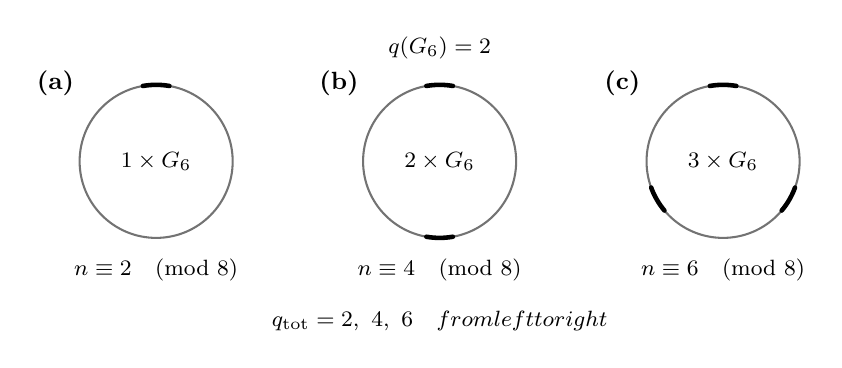
\begin{tikzpicture}[
  x=0.90cm,
  y=0.90cm,
  line cap=round,
  line join=round,
  ring/.style={draw=black!55,line width=0.75pt},
  defect/.style={draw=black,line width=1.65pt},
  panel/.style={font=\small\bfseries},
  label/.style={font=\footnotesize,align=center}
]
  \node[label] at (6.0,4.05) {$q(G_6)=2$};
  \node[panel] at (0.58,3.55) {(a)};
  \node[panel] at (4.58,3.55) {(b)};
  \node[panel] at (8.58,3.55) {(c)};
  \foreach \cx/\count/\residue in {
    2.0/1/2,
    6.0/2/4,
    10.0/3/6
  } {
    \draw[ring] (\cx,2.45) circle (1.08);
    \foreach \j in {1,...,\count} {
      \pgfmathsetmacro{\ang}{90+360*(\j-1)/\count}
      \pgfmathsetmacro{\startang}{\ang-10}
      \pgfmathsetmacro{\endang}{\ang+10}
      \draw[defect]
        ({\cx+1.08*cos(\startang)},{2.45+1.08*sin(\startang)})
        arc[start angle=\startang,end angle=\endang,radius=1.08];
    }
    \node[label] at (\cx,2.45) {$\count\times G_6$};
    \node[label] at (\cx,0.92)
      {$n\equiv\residue\pmod 8$};
  }
  \node[label] at (6.0,0.20)
    {$q_{\mathrm{tot}}=2,\ 4,\ 6\quad\text{from left to right}$};
\end{tikzpicture}
